\documentclass[12pt,a4paper,answers]{exam} % Adds 'answers' to print solutions, 'cancelspace' to avoid blank space when solutions provided but 'answers' not set.
\usepackage[utf8]{inputenc}
\usepackage{multicol}
\usepackage[left=1cm,right=1cm,top=1.5cm,bottom=1.8cm]{geometry}
\usepackage{amsmath,amsthm,amsfonts,amssymb,mathtools}
\usepackage{color,graphicx}
\graphicspath{ {figures/} }
\usepackage{todonotes}
\usepackage{xfrac}
\usepackage{hyperref}
\usepackage{subfig}
\usepackage{tabu}

% Style
% Cheatsheet style

\usepackage{ifthen}
\usepackage{listings}

% This sets page margins to .5 inch if using letter paper, and to 1cm
% if using A4 paper. (This probably isn't strictly necessary.)
% If using another size paper, use default 1cm margins.
\ifthenelse{\lengthtest{\paperwidth = 11in}}
  % Then
  { \geometry{top=.5in,left=.5in,right=.5in,bottom=.5in} }
  % Else
  { \ifthenelse{\lengthtest{\paperwidth = 297mm}}
    {\geometry{top=1.5cm,left=0.3cm,right=0.3cm,bottom=0.8cm} }
  }

% Redefine section commands to use less space
\makeatletter
\renewcommand{\section}{\@startsection{section}{1}{0mm}%
                                {-1ex plus -.5ex minus -.2ex}%
                                {0.5ex plus .2ex}%x
                                {\color{darkred}\normalfont\large\bfseries}}
\renewcommand{\subsection}{\@startsection{subsection}{2}{0mm}%
                                {-1explus -.5ex minus -.2ex}%
                                {0.5ex plus .2ex}%
                                {\color{darkdarkred}\normalfont\normalsize\bfseries}}
\renewcommand{\subsubsection}{\@startsection{subsubsection}{3}{0mm}%
                                {-1ex plus -.5ex minus -.2ex}%
                                {1ex plus .2ex}%
                                {\normalfont\small\bfseries}}
\makeatother

% Define BibTeX command
\def\BibTeX{{\rm B\kern-.05em{\sc i\kern-.025em b}\kern-.08em
    T\kern-.1667em\lower.7ex\hbox{E}\kern-.125emX}}

% Don't print section numbers
\setcounter{secnumdepth}{0}

\setlength{\parindent}{0pt}
\setlength{\parskip}{0pt plus 0.5ex}

% Setting colors
\definecolor{lightgray}{rgb}{0.7,0.7,0.7}
\definecolor{lightergray}{rgb}{0.9,0.9,0.9}
\definecolor{darkblue}{rgb}{0.4,0.4,1}
\definecolor{darkred}{rgb}{0.9,0.2,0.2}
\definecolor{darkdarkred}{rgb}{0.6,0.0,0.0}
\definecolor{lightred}{rgb}{1,0.6,0.6}
\definecolor{lightgreen}{rgb}{0.6,1,0.6}
\definecolor{lightblue}{rgb}{0.6,0.8,1}
\definecolor{darkgreen}{rgb}{0.4,1,0.4}

% Set code listing style
\lstset {
    backgroundcolor=\color{lightgray},
    basicstyle=\ttfamily\scriptsize,
    breaklines=true,
}

\lstdefinestyle{bb}{
    backgroundcolor=\color{lightergray},
    frame=L,
    xleftmargin=\parindent,
}

% Remove `itemize` indentation
\usepackage{enumitem}
\setlist[itemize]{leftmargin=*}
\setitemize{noitemsep,topsep=0pt,parsep=0pt,partopsep=0pt}

% Set hyperlink style
\hypersetup{hidelinks}

% Enable figures
\newenvironment{colfig}
  {\par\medskip\noindent\minipage{\columnwidth}\centering}
  {\endminipage\par\medskip}
  
% Enable tables
\newenvironment{coltab}
  {\par\bigskip\noindent\minipage{\columnwidth}\centering}
  {\endminipage\par\bigskip}

% Enable arg min/max math operators
\DeclareMathOperator*{\argmin}{arg\,min}
\DeclareMathOperator*{\argmax}{arg\,max}

\newcommand{\by}{by}
\newcommand{\of}{of}
\newcommand{\epfl}{EPFL}


\newcommand{\school}{IC}
\newcommand{\courseId}{CS-423}
\newcommand{\courseTitle}{Distributed information systems}
\newcommand{\courseUrl}{http://isa.epfl.ch/imoniteur_ISAP/!GEDPUBLICREPORTS.pdf?ww_i_reportModel=1696552884&ww_i_reportModelXsl=1696552963&ww_i_itemplan=1799090851&ww_c_langue=en}
\newcommand{\staff}{\href{http://people.epfl.ch//karl.aberer}{Prof. K. Aberer}}
\newcommand{\academicYear}{2014-2015}
\newcommand{\academicSemester}{Spring}
\newcommand{\lastUpdate}{\today}
\newcommand{\version}{1.0}

\author{Marc Bourqui}
\title{Distributed Information Systems\\Class questions}

\pdfinfo{
  /Title (Distributed information systems class questions)
  /Creator (TeX)
  /Producer (pdfTeX 1.40.0)
  /Author (\author)
  /Subject (Distributed information systems class questions)
  /Keywords (distributed, information, systems, quiz, question)
}

\newcommand{\mat}[1]{\ensuremath{\textbf{#1}}}

\pagestyle{headandfoot}
\runningheader{}
{
\includegraphics[width=0.6cm]{epfl.png}\ \epfl\ - \school\ - \href{\courseUrl}{\courseId\ \textbf{\courseTitle}}\ \by\ \textit{\staff}\ - \academicSemester\ \academicYear}
{}
\runningheadrule
\runningfootrule
\runningfooter{}{\thepage}{Version \version\ \of\ \lastUpdate}

% Change the default list settings
\renewcommand{\checkboxeshook}{%
\setlength{\leftmargin}{0.5cm}%
}

\begin{document}
\maketitle
%\setlength{\headsep}{-1cm}

\begin{flushleft}
\raggedright
\footnotesize
\sffamily

\begin{multicols*}{2}

% multicol parameters
% These lengths are set only within the two main columns
%\setlength{\columnseprule}{0.25pt}
\setlength{\premulticols}{1pt}
\setlength{\postmulticols}{1pt}
\setlength{\multicolsep}{1pt}
\setlength{\columnsep}{2cm}



\begin{questions}
\part{Introduction}
% -------------------------------------------------------------------------------------------------

\section{An Overview}
\subsection{Information Systems (Week~1)}
% 13
\question Functions in models
\begin{checkboxes}
\choice Are always computable
\choice Can always be represented as data
\CorrectChoice Can be constrained by axioms
\end{checkboxes}

% 13
\question Interpretation relationships
\begin{checkboxes}
\choice Are always computable
\CorrectChoice Relate constants to real-world entities
\choice Are uniquely defined
\end{checkboxes}


\subsection{Data Management}

% 27
\question What is not specified in the data definition language~?
\begin{checkboxes}
\choice The structure of a relational table
\CorrectChoice The query of user
\choice A constraint on a relational table
\end{checkboxes}

% 28
\question Logical data independence means
\begin{checkboxes}
\choice An abstract data type is implemented using different data structures
\CorrectChoice A new view is computed without changing an existing database schema
\choice A model can be represented in different data modelling formalisms
\end{checkboxes}


\subsection{Data Management Tasks}

% 39 4
\question Which is wrong~? An index structure
\begin{checkboxes}
\choice Is created as part of physical database design
\choice Is selected during query optimization
\choice Accelerates search queries
\CorrectChoice Accelerates tuple insertion
\end{checkboxes}

% 40 2
\question Persistence means that
\begin{checkboxes}
\choice A change of a transaction on a database is never lost after it is completed
\CorrectChoice The state of a database is independent of the lifetime of a program
\choice The same logical database can be stored in different ways on a storage medium
\end{checkboxes}


\subsection{Information Management}

% 49 2
\question Grouping Twitter users according to their interest by analyzing the content of their tweets is
\begin{checkboxes}
\choice A retrieval task
\CorrectChoice A data mining task
\choice An evaluation task
\choice A monitoring task
\end{checkboxes}


\subsection{Distributed Information Systems}

% 55 2
\question Creating a web portal for comparing product prices is (primarily) a problem of
\begin{checkboxes}
\choice Distributed data management
\CorrectChoice Heterogeneous data integration
\choice Collaboration among autonomous systems
\end{checkboxes}


\subsection{Distributed Data Management}

% 62 4
\question If Google retrieves the result of a search of a Swiss client from a US server and stores it subsequently on a Swiss server, it is doing
\begin{checkboxes}
\choice Distributed query processing
\choice Data partitioning
\choice Data replication
\CorrectChoice Data caching
\end{checkboxes}

% 68 1
\question When you open a Web page with an embedded Twitter stream, the communication model used by Twitter is
\begin{checkboxes}
\CorrectChoice Push, unicast and conditional
\choice Pull, multicast and ad-hoc
\choice Push, multicast and ad-hoc
\choice Pull, unicast and conditional
\end{checkboxes}


\subsection{Heterogeneity}

% 79 3
\question Creating a web portal for comparing product prices requires to address
\begin{checkboxes}
\choice Syntactic heterogeneity
\choice Semantic heterogeneity
\CorrectChoice Both
\end{checkboxes}

% 80 5
\question An \emph{ontology} is a
\begin{checkboxes}
\choice Database
\choice Database schema
\choice Data model
\choice Data modeling formalism
\CorrectChoice Model
\end{checkboxes}


\subsection{Autonomy}

% 89
\question \emph{Trust} is
\begin{checkboxes}
\choice A quality of information
\choice A quality of a user
\choice A quality of the relationship among user and information
\choice A quality of the relationship among users
\end{checkboxes}



\part{Storage}
% -------------------------------------------------------------------------------------------------
\section{Distributed Data Management}

\subsection{Schema Fragmentation}
\subsubsection{Relational Databases}

%9
\question At which phase of the database lifecycle is fragmentation performed ?
\begin{checkboxes}
\CorrectChoice At database design time
\choice During distributed query processing
\choice During updates to a distributed database
\end{checkboxes}

%10
\question The reconstruction property expresses that
\begin{checkboxes}
\choice In case of a node failure the data can be recovered from a fragment from another node
\CorrectChoice The original data can be fully recovered from the fragments
\choice Every data value of the original data can be found in at least one fragment
\end{checkboxes}



\subsubsection{Primary Horizontal Fragmentation (Week~2)} %Week2

%16
\question Example: application A1 accesses
\begin{colfig}
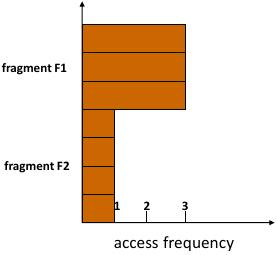
\includegraphics[scale=0.5]{w2_s16}
\end{colfig}
\begin{enumerate}
\item Fragment F1: with frequency 3
\item Fragment F2: with frequency 1
\end{enumerate}
A1 accesses the whole relation with frequency
\begin{checkboxes}
\CorrectChoice $\sfrac{13}{7}$
\choice $\sfrac{4}{7}$
\choice $\sfrac{14}{7}$
\end{checkboxes}

%26
\question Consider the access frequencies below: 
\begin{coltab}
\begin{tabu}{X[cm]|*{4}{X[cm]}}
$<$af1,af2$>$ & \texttt{Location = "Paris"} & \texttt{Location = "Geneva"}  & \texttt{Location = "Munich"} & \texttt{Location = "Bangalore"} \\
\hline
\hline
\texttt{Budget > 200000} & $<3,1>$ & $<3,1>$ & $<1,3>$ & n/a \\
\texttt{Budget <= 200000} & $<1,1>$ & $<1,1>$ & n/a & $<1,3>$ \\
\hline
\end{tabu}
\end{coltab}
\begin{parts}
\part How many horizontal fragments would a minimal and complete fragmentation have?
\begin{checkboxes}
\CorrectChoice 3
\choice 4
\choice 6
\end{checkboxes}

%27
\part Which of the following sets of simple predicates is complete?
%\missingfigure{table} %Same as above
\begin{checkboxes}
\choice {Location = ”Munich", Budget \textgreater\ 200000 }
\choice {Location = ”Munich", Location = ”Bangalore”}
\choice {Location = ”Paris", Budget $\le$ 200000 }
\CorrectChoice None of those
\end{checkboxes}
\end{parts}

%33
\question Which is true for MinFrag algorithm?
\begin{checkboxes}
\choice The output is independent of the order of the input
\choice It produces a monotonically increasing set of predicates
\CorrectChoice It always terminates
\choice All of the above statements are true
\end{checkboxes}


%39
\question When deriving a horizontal fragmentation for relation $S$ from a horizontally fragmented relation $R$
\begin{checkboxes}
\CorrectChoice Some primary key attribute in $R$ must be a foreign key in $S$
\choice Some primary key attribute in $S$ must be a foreign key in $R$
\choice Both are required
\end{checkboxes}



\subsection{Graph Databases} %Week3
\subsubsection{Semi-structured Data (Week~3)}

%14
\question Semi-structured data
\begin{checkboxes}
\choice Is always schema-less
\CorrectChoice Always embeds schema information into the data
\choice Must always be hierarchically structured
\choice Can never be indexed
\end{checkboxes}

%15
\question Why is XML a document model?
\begin{checkboxes}
\choice It supports application-specific markup
\choice It supports domain-specific schemas
\CorrectChoice It has a serialized representation
\choice It uses HTML tags
\end{checkboxes}


\subsubsection{Graph Data Model}

%22
\question In a graph database
\begin{checkboxes}
\choice There is a unique root node
\CorrectChoice Each node has a unique identifier
\choice Data values in leaf nodes are unique
\choice The labels of edges leaving a node are different
\choice There is a unique path from the root to each leaf
\end{checkboxes}

%36
\question The simulation relationship is a relation
\begin{checkboxes}
\CorrectChoice Among nodes in the data and schema graph
\choice Among edges in the data and schema graph
\choice Among sets of nodes in the data and schema graph
\choice Among sets of edges in the data and schema graph
\end{checkboxes}

%37
\question Which is true?
\begin{checkboxes}
\choice For each labelled edge in $S$ a corresponding edge in $D$ can be identified
\choice For each root node in $S$ a corresponding root node $D$ can be identified
\CorrectChoice For each leaf node in $D$ a corresponding typed node in $S$ can be identified
\choice For each node in $S$ a unique path reaching it from a root node can be identified
\end{checkboxes}

%43
\question If there exists a uniquely defined simulation relationship among a graph database $D$ and a schema graph $S$
\begin{checkboxes}
\choice The data and schema graph are simulation equivalent
\CorrectChoice Ambiguous classification cannot occur
\choice Multiple classification cannot occur
\end{checkboxes}

%48
\question If schema graph $S_1$ subsumes $S_2$
\begin{checkboxes}
\choice Every graph database corresponding to $S_1$ corresponds also to $S_2$
\CorrectChoice $S_2$ simulates $S_1$
\choice $S_1$ has fewer nodes than $S_2$
\end{checkboxes}


\subsubsection{Schema Extraction}

%57
\question Which is wrong? In a dataguide
\begin{checkboxes}
\choice Every path in the data graph occurs only once
\CorrectChoice Every node in the data graph occurs only in one data guide node
\choice Every data guide node has a unique set of nodes
\choice A leaf node in the data graph corresponds always to a leaf node in the data guide
\end{checkboxes}

%63
\question In a non-deterministic schema graph
\begin{checkboxes}
\CorrectChoice Every node of the data graph occurs exactly once
\choice Every path of the data graph occurs at most once
\choice Every label of an outgoing edge of a node in the schema graph is unique
\end{checkboxes}



\part{Search}
% -------------------------------------------------------------------------------------------------
\section{Information Retrieval and Data Mining}
\subsection{Information Retrieval} %Week4
\subsubsection{Information Retrieval (Week~4)}

%12
\question A retrieval model attempts to model
\begin{checkboxes}
\choice The interface by which a user is accessing information
\CorrectChoice The importance a user gives to a piece of information
\choice The formal correctness of a query formulation by user
\choice All of the above
\end{checkboxes}

%16
\question If the top 100 documents contain 50 relevant documents
\begin{checkboxes}
\choice The precision of the system at 50 is 0.5
\CorrectChoice The precision of the system at 100 is 0.5
\choice The recall of the system is 0.5
\choice None of the above
\end{checkboxes}

%17
\question If retrieval system A has a higher precision than system B
\begin{checkboxes}
\choice The top k documents of A will have higher similarity values than the top k documents of B
\CorrectChoice The top k documents of A will contain more relevant documents than the top k documents of B
\choice A will recall more documents above a given similarity threshold than B
\choice Relevant documents in A will have higher similarity values than in B
\end{checkboxes}


\subsubsection{Text-based Information Retrieval}

%25
\question Full-text retrieval means that
\begin{checkboxes}
\choice The document text is grammatically deeply analyzed for indexing
\choice The complete vocabulary of a language is used to extract index terms
\CorrectChoice All words of a text are considered as potential index terms
\choice All grammatical variations of a word are indexed
\end{checkboxes}

%26
\question The term-document matrix indicates
\begin{checkboxes}
\CorrectChoice How many relevant terms a document contains
\choice How relevant a term is for a given document
\CorrectChoice How often a relevant term occurs in a document collection
\CorrectChoice Which relevant terms are occurring in a document collection
\end{checkboxes}

%31
\question Let the query be represented by the following vectors:
(1, 0, -1) (0, -1, 1); the document by the vector (1, 0, 1)
\begin{checkboxes}
\choice Matches the query because it matches the first query vector
\CorrectChoice Matches the query because it matches the second query vector
\choice Does not match the query because it does not match the first query vector
\choice Does not match the query because it does not match the second query vector
\end{checkboxes}

%38
\question Which is right? The term frequency is normalized
\begin{checkboxes}
\CorrectChoice By the maximal frequency of a term in the document
\choice By the maximal frequency of a term in the document collection
\choice By the maximal frequency of a term in the vocabulary
\choice By the maximal term frequency of any document in the collection
\end{checkboxes}


%44
\question The inverse document frequency of a term can increase
\begin{checkboxes}
\choice By adding the term to a document that contains the term
\CorrectChoice By adding a document to a document collection that does not
contain the term
\choice By removing a document from the document collection that
does not contain the term
\choice By adding a document to a document collection that contains
the term
\end{checkboxes}



\subsection{Advanced Retrieval Models} % Week 5

\subsubsection{Latent Semantic Indexing (Week~5)}


% 13 1
\question In vector space retrieval each row of the matrix $\mat{M}^T$ corresponds to
\begin{checkboxes}
\CorrectChoice A document
\choice A concept
\choice A query
\choice A query result
\end{checkboxes}

% 22 2
\question Applying SVD to a term-document matrix \mat{M}. Each concept is represented
\begin{checkboxes}
\choice As a singular value
\CorrectChoice As a linear combination of terms of the vocabulary
\choice As a linear combination of documents in the document collection
\choice As a least square approximation of the matrix \mat{M}
\end{checkboxes}

% 23 2
\question The number of term vectors in the SVD for LSI
\begin{checkboxes}
\choice Is smaller than the number of rows in the matrix \mat{M}
\CorrectChoice Is the same as the number of rows in the matrix \mat{M}
\choice Is larger than the number of rows in the matrix \mat{M}
\end{checkboxes}

% 32 1
\question A query transformed into the concept space for LSI has
\begin{checkboxes}
\CorrectChoice $s$ components (number of singular values)
\choice $m$ components (size of vocabulary)
\choice $n$ components (number of documents)
\end{checkboxes}


\subsubsection{User Relevance Feedback}

% 40 3
\question Can documents which do not contain any keywords of the original query receive a positive similarity coefficient after relevance feedback ?
\begin{checkboxes}
\choice No
\choice Yes, independent of the values $\beta$ and $\gamma$
\CorrectChoice Yes, but only if $\beta>0$
\choice Yes, but only if $\gamma>0$
\end{checkboxes}


\subsubsection{Link-based Ranking}

% 49 1,3
\question A positive random jump value for exactly one node implies that
\begin{checkboxes}
\CorrectChoice a random walker can leave the node even without outgoing edges
\choice a random walker can reach the node multiple times even without outgoing edges
\CorrectChoice a random walker can reach the node even without incoming edges
\choice none of the above
\end{checkboxes}

% 56 3
\question Given the graph below and an initial hub vector of $(1,1,1)$. The hub-authority ranking will result in the following
\begin{colfig}
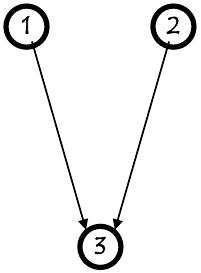
\includegraphics[scale=0.3]{w5_s56}
\end{colfig}
\begin{checkboxes}
\choice authority vector $(0,0,1$)~; hub vector $(1,1,0)$
\choice authority vector $(0,0,2)$~; hub vector $(2,2,0)$
\CorrectChoice authority vector $(0,0,1)$~; hub vector $(\frac{1}{2},\frac{1}{2},0)$
\choice authority vector $(0,0,2)$~; hub vector $(1,1,0)$
\end{checkboxes}


\subsubsection{Inverted Files (Week~6)}

% 10 3
\question A posting indicates
\begin{checkboxes}
\choice The frequency of a term in the vocabulary
\choice The frequency of a term in a document
\CorrectChoice The occurrence of a term in a document
\choice The list of terms occurring in a document
\end{checkboxes}

% 11 4
\question When indexing a document collection using an inverted file, the main space requirement is implied by
\begin{checkboxes}
\choice The access structure
\choice The vocabulary
\choice The index file
\CorrectChoice The postings file
\end{checkboxes}

% 18 4
\question Using a trie in index construction
\begin{checkboxes}
\choice Helps to quickly find words that have been seen before
\choice Helps to quickly decide whether a word has not been seen before
\choice Helps to maintain the lexicographic order of words seen in the documents
\CorrectChoice All of the above
\end{checkboxes}

% 25 1
\question Maintaining the order of document identifiers when partitioning the document collection is important
\begin{checkboxes}
\CorrectChoice In the index merging approach for single node machines
\choice In the map-reduce approach for parallel clusters
\choice In both
\choice In neither of the two
\end{checkboxes}


\subsubsection{Distributed Retrieval}

% 36 2
\question When applying Fagin’s algorithm for a query with three different terms for finding the $k$ top documents, the algorithm will scan
\begin{checkboxes}
\choice 2 different lists
\CorrectChoice 3 different lists
\choice $k$ different lists
\choice it depends how many rounds are taken
\end{checkboxes}

% 37 2
\question Once $k$ documents have been identified that occur in all of the lists
\begin{checkboxes}
\choice These are the top-$k$ documents
\CorrectChoice The top-$k$ documents are among the documents seen so far
\choice The search has to continue in round-robin till the top-$k$ documents are identified
\choice Other documents have to be searched to complete the top-$k$ list
\end{checkboxes}


\section{Peer-2-Peer Search}
\subsection{Peer-2-Peer Systems}
\subsubsection{P2P Systems and Resource Location (Week~7)}

% 11 2
\question Which resource is in Napster not shared in a P2P approach~?
\begin{checkboxes}
\choice File storage
\CorrectChoice File metadata storage
\choice Network bandwidth
\choice Content rights
\end{checkboxes}

% 18 1
\question "Churn" refers to the fact that in a peer-to-peer system~:
\begin{checkboxes}
\CorrectChoice Peers constantly join and leave the network
\choice Peers constantly add and remove resources
\choice Peers constantly search for resources
\end{checkboxes}

% 19 2
\question An "overlay network" supports~:
\begin{checkboxes}
\choice Efficient routing to a given IP address
\CorrectChoice Efficient routing to the location of a resource identifier
\choice Efficient exchange of large files
\choice Efficient messaging in centralized social network
\end{checkboxes}


\subsubsection{Unstructured P2P Overlay Networks}

% 26 2
\question In an unstructured overlay network (such as Gnutella) a peer receiving a "peer discovery" message (ping)
\begin{checkboxes}
\choice Responds by sending a message to the originator of the message
\CorrectChoice Responds by replying to the last forwarder of the message
\choice Responds by sending a message to all its neighbors
\end{checkboxes}

% 31 3
\question If the largest city in the world has 16 Mio inhabitants, the second largest 11.3 Mio inhabitants, the third largest 9.2 Mio, the fourth largest 8.0 Mio, and so on, then this is
\begin{checkboxes}
\choice A Powerlaw distribution
\CorrectChoice A Zipf distribution
\choice None of the two
\end{checkboxes}

% 32 2
\question Assume that in a country the size of cities follows a powerlaw distribution with exponent 2. A city of 16 Mio inhabitants has probability of $\sfrac{1}{256}$ to occur. Then a city of 8 Mio inhabitants is
\begin{checkboxes}
\choice Twice as probable
\CorrectChoice Four times as probable
\choice Eight times as probable
\end{checkboxes}

% 42 1
\question Expanding ring search is particularly suitable to locate
\begin{checkboxes}
\CorrectChoice Frequent items
\choice Rare items
\choice Does not matter
\end{checkboxes}

% 43 2
\question With the square root rule for replica allocation~: given two items that are accessed with probabilities $p_1 > p_2$ that are replicated $r_1$ and $r_2$ times. Which is always true~?
\begin{checkboxes}
\choice $r_1 < r_2$
\CorrectChoice $\sfrac{r1}{p1} < \sfrac{r2}{p2}$
\choice $r_1 - p_1 < r_2 – p_2$
\end{checkboxes}


%\subsubsection{Hierarchical P2P Overlay Networks}
% no question

\subsubsection{Hierarchical P2P Overlay Networks (Week~8)}

% 14 1
\question The index information in a structured overlay network
\begin{checkboxes}
\CorrectChoice Provides references to route a search request within the overlay network
\choice Provides for a given key the reference to the peer that stores the resource
\choice Is replicated in routing tables to support redundant search paths
\end{checkboxes}

% 14 1
\question For the given routing table, the search request for the key 0101 is routed
\begin{colfig}
\centering
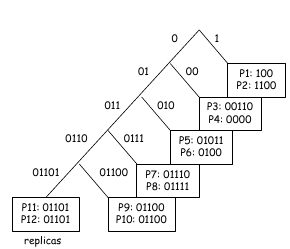
\includegraphics[scale=0.75]{w8_s14}
\end{colfig}

\begin{checkboxes}
\CorrectChoice Always to peer $P_5$
\choice Either to peer $P_5$ or $P_6$
\choice Either to peer $P_3$, $P_4$, $P_5$ or $P_6$
\end{checkboxes}

% 22 1
\question When routing in Chord
\begin{checkboxes}
\CorrectChoice The next hop is always uniquely determined
\choice The next hop can be chosen among a constant number of possible candidates
\choice The next hop can be chosen among $\log n$ possible candidates
\end{checkboxes}

% 23 4
\question When adding $q$ to the Chord ring~: in the routing table of $p$
\begin{colfig}
\begin{minipage}[c]{0.45\linewidth}
\centering
\begin{tabular}{c|c}
\hline
$i$ & $s_i$\\
\hline
\hline
1 & $p_2$\\
2 & $p_2$\\
3 & $p_2$\\
4 & $p_3$\\
5 & $p_4$\\
\hline
\end{tabular}
\end{minipage}
\begin{minipage}[c]{0.45\linewidth}
\centering
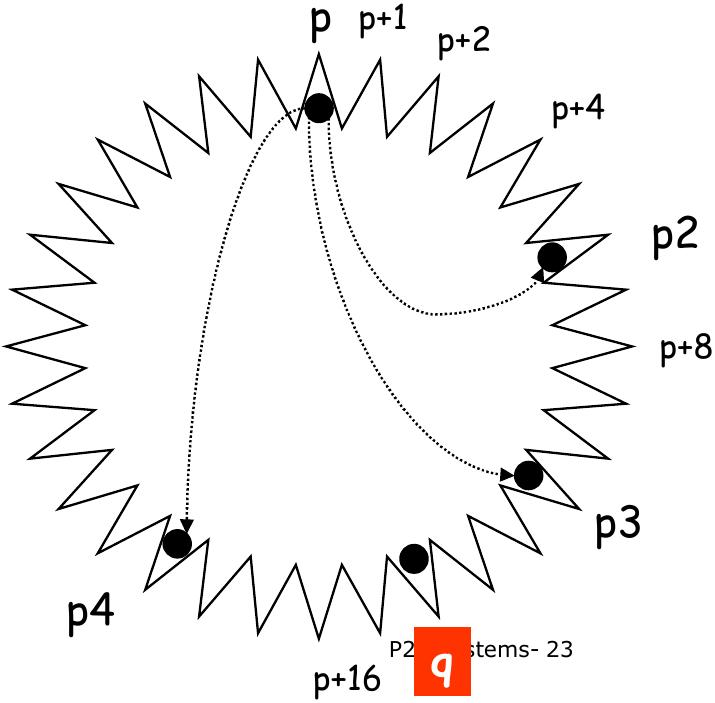
\includegraphics[width=\textwidth]{w8_s23}
\end{minipage}
\end{colfig}
\begin{checkboxes}
\choice Entries for $i=1,2,3,4$ change
\choice The entry for $i=4$ changes
\choice The entry for $i=5$ changes
\CorrectChoice No entry changes
\end{checkboxes}

% 31 1
\question When adding $n$ peers to CAN the number of new zones
\begin{checkboxes}
\CorrectChoice Is exactly $n$
\choice It depends what the keys of the peers were
\choice It depends on the dimensionality of the key space
\end{checkboxes}
\begin{solution}
One zone per new peer.
\end{solution}

% 32 3
\question In CAN, for a fixed dimensionality $d>2$, when moving from 1 to 2 realities
\begin{checkboxes}
\choice  The number of entries in the routing table increases by 2
\choice The number of entries in the routing table increases by $d$
\CorrectChoice The number of entries in the routing table doubles
\end{checkboxes}

% 41 2
\question In FreeNet the routing table is updated
\begin{checkboxes}
\choice When a search request message arrives
\CorrectChoice When a query answer message arrives
\choice When an insert file message arrives
\end{checkboxes}

% 42 1
\question For which of the following structured overlay networks the length of a search path is always guaranteed to be shorter than the length of the longest key
\begin{checkboxes}
\CorrectChoice P-Grid
\choice CAN
\choice FreeNet
\end{checkboxes}
% Based on the path of the key itself

% 52 2
\question The local clustering coefficient is the probability that two of my friends are also friends. If I have 10 friends and among them 15 friendships exist, my local clustering coefficient is
\begin{checkboxes}
\choice $\sfrac{1}{6}$
\CorrectChoice $\sfrac{1}{3}$
\choice $\sfrac{2}{3}$
\choice $\sfrac{3}{2}$
\end{checkboxes}
\begin{solution}
Look at the formula in the slides notes.
\end{solution}

% 53 3
\question A random graph has
\begin{checkboxes}
\choice High clustering and low diameter
\choice High clustering and high diameter
\CorrectChoice Low clustering and low diameter
\choice Low clustering and high diameter
\end{checkboxes}

% 66 1
\question In a three-dimensional Kleinberg small world network with $\log n$ long range links the search cost is
\begin{checkboxes}
\CorrectChoice $\log n$
\choice $\log^2 n$
\choice $\log^3 n$
\end{checkboxes}

\part{Dissemination}
\section{Data Broadcasting in Mobile Networks (Week~9)}

% 11 3
\question Latency is
\begin{checkboxes}
\choice The time a client is connected to a broadcast channel
\choice The time a client listens actively on a broadcast channel
\CorrectChoice The time a client waits for receiving a data item on a broadcast channel 
\end{checkboxes}

% 12 2
\question Data Broadcast is beneficial when
\begin{checkboxes}
\choice Clients have a high upstream bandwidth
\CorrectChoice Many clients are interested in the same information
\choice Clients have many different requests
\end{checkboxes}

% 20 1
\question Assume the broadcast channel has one item accessed with frequency 9 and three others accessed with frequency 1. The expected delay for accessing the first item in an optimal broadcast organization will be
\begin{checkboxes}
\CorrectChoice 1
\choice 2
\choice 3
\end{checkboxes}

% 21 2
\question Assume the broadcast channel has one item accessed with frequency 9 and three others accessed with frequency 1. The expected delay for accessing the second type of items will be
\begin{checkboxes}
\choice 1
\CorrectChoice 3
\choice 6
\end{checkboxes}

% 34 2
\question When organizing a broadcast disk a "chunk"
\begin{checkboxes}
\choice Contains always all elements of the broadcast disk
\CorrectChoice Contains sometimes all elements of the broadcast disk
\choice Contains never all elements of the broadcast disk
\end{checkboxes}

% 35 1,3
\question When organizing a broadcast disk, which is true~?
\begin{checkboxes}
\CorrectChoice The number of copies of different chunks in a broadcast disk is constant
\choice The number of copies of different data items in a broadcast disk is constant
\CorrectChoice The number of data items in the chunks of one disk is constant
\choice The data items in the chunks of one disk are always the same
\end{checkboxes}

% 48 1,2,3 
\question Which is true~?
\begin{checkboxes}
\CorrectChoice LRU (least recently used) is not optimal because it does not consider the frequency of data items in a data broadcast
\CorrectChoice MPA (most probable accessed) is not optimal because it does not consider the frequency of data items in a data broadcast
\CorrectChoice Only PIX considers the frequency of data items in a data broadcast
\end{checkboxes}

% 49 2
\question Assume the broadcast and access pattern below. Assuming that $c=\sfrac{1}{2}$ what is the access frequency estimate for B at time 6~?
\begin{colfig}
\centering
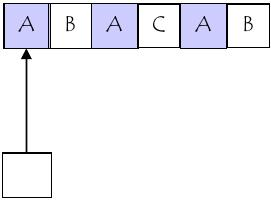
\includegraphics[scale=0.75]{w9_s49}
\end{colfig}
\begin{checkboxes}
\choice \sfrac{1}{3}
\CorrectChoice \sfrac{1}{4}
\choice \sfrac{1}{6}
\choice \sfrac{1}{12}
\end{checkboxes}
\begin{solution}

At $t_2$, B has value $\frac{\sfrac{1}{2}}{2-0}+0 = \frac{1}{4}$.\\
At $t_6$, B has value $\frac{\sfrac{1}{2}}{6-2}+\frac{1}{2}\cdot\frac{1}{4} = \frac{1}{4}$
\end{solution}

% 60 1
\question The minimal latency of a broadcast channel can be achieved
\begin{checkboxes}
\CorrectChoice By not indexing the broadcast
\choice By indexing the broadcast only once
\choice By indexing the broadcast according to the (1,m) rule
\end{checkboxes}

% 61 2
\question The term "probe wait" refers to
\begin{checkboxes}
\choice The time for waiting for a data page
\CorrectChoice The time for waiting for an index segment
\choice The time for waiting for a data segment
\end{checkboxes}

\part{Big Data Analytics}
\section{Association Rules (Week~10)}
% 15 2
\question Based on the analysis of search terms and subsequent link clicks, a search engine provider places ads on  search results that are most likely to be clicked by the users.
This task is an example of~:
\begin{checkboxes}
\choice Local rule discovery
\CorrectChoice Predictive modelling
\choice Descriptive modelling
\choice Exploratory data analysis
\end{checkboxes}

\subsection{Pattern structure}
% 22 4
\question Let’s assume that the transactions are stored in a relation $T(x, A1, \ldots, A5)$, where $x$ is the customer and each attribute $A1, \ldots, A5$ can have 3 different values. How many different items exist after reduction to a single dimension~?
\begin{checkboxes}
\choice 5
\choice 243
\choice 125
\CorrectChoice 15
\end{checkboxes}

\subsection{Scoring function}
% 28 3
\question 10 itemsets out of 100 contain item A, of which 5 also contain B. The rule A$\rightarrow$ B has~:
\begin{checkboxes}
\choice 5\% support and 10\% confidence
\choice 10\% support and 50\% confidence
\CorrectChoice 5\% support and 50\% confidence
\choice 10\% support and 10\% confidence
\end{checkboxes}
\begin{solution}
5/100 transactions which have A and B support, confidence half of the time we buy B when we buy A
\end{solution}

% 29 4
\question 10 itemsets out of 100 contain item A, of which 5 also contain B. The rule B$\rightarrow$A has~:
\begin{checkboxes}
\choice unknown support and 50\% confidence
\choice unknown support and unknown confidence
\choice 5\% support and 50\% confidence
\CorrectChoice 5\% support and unknown confidence
\end{checkboxes}

% 42 3
\question Given the frequent 2-itemsets \{1,2\}, \{1,4\}, \{2,3\} and \{3,4\}, how many 3-itemsets are generated and how many are pruned~?
\begin{checkboxes}
\choice 2, 2
\choice 1, 0
\CorrectChoice 1, 1
\choice 2, 1
\end{checkboxes}

% 43 2
\question After the join step, the number of $k+1$-itemsets \ldots
\begin{checkboxes}
\choice is equal to the number of frequent $k$-itemsets
\CorrectChoice can be equal, lower or higher than the number of frequent $k$-itemsets
\choice is always higher than the number of frequent $k$-itemsets
\choice is always lower than the number of frequent $k$-itemsets
\end{checkboxes}
\begin{solution}
\{1,2,3\}, \{1,2,4\} $\rightarrow$ \{1,2,3,4\}\\
\{1,2,5\} $\rightarrow$ \{1,2,3,5\},\{1,2,4,5\}
\end{solution}

% 46 1
\question If rule \{A,B\}$\rightarrow$\{C\} has confidence $c_1$ and rule \{A\}$\rightarrow$\{C\} has confidence $c_2$ , then \ldots
\begin{checkboxes}
\choice $c_2 \geq c_1$
\CorrectChoice $c_1 > c_2$ and $c_2 > c_1$ are both possible
\choice $c_1 \geq c_2$
\end{checkboxes}
\begin{solution}
Typo in the slides, meant \{A\}$\rightarrow$\{B,C\}
% Ex fromn Roger Vion
%1. transactions : {A}, {A, B}, {A, B, C}
%=> c1 = 1/2 > c2 = 1/3
%
%2. transactions : {A}, {A, B}, {A, C}, {A, B, C}
%=> c1 = 1/2 = c2
%
%3. transactions : {A, B}, {A, C}, {A, B, C}
%=> c1 = 1/2 < c2 = 2/3
\end{solution}


\subsection{Clustering \& Classification (Week 11)}
\subsection{Clustering}
% 14 4
\question Suppose we have a dataset of pictures and we want to cluster them. Which partitioning algorithm seems more appropriate?
\begin{colfig}
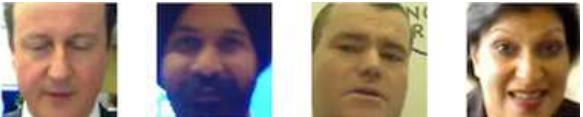
\includegraphics[scale=0.3]{w11_s13}
\end{colfig}
\begin{checkboxes}
\choice k-medoids
\choice k-medians
\choice k-means
\CorrectChoice none of the above
\end{checkboxes}

\subsubsection{Classification}
% 
\question What will be the color of the middle points after convergence?
\begin{colfig}
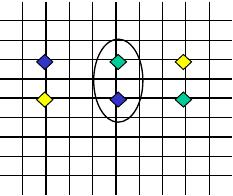
\includegraphics[scale=0.3]{w11_s20}
\end{colfig}
\begin{checkboxes}
\choice Green
\choice Yellow
\choice Blue
\choice k-means does not converge
\end{checkboxes}

% 27 3
\question If a classifier has 75\% accuracy, it means that \ldots
\begin{checkboxes}
\choice correctly classifies 75\% of the data items in the training set
\choice It correctly classifies 100\% of the data items in the training set but only 75\% in the test set
\CorrectChoice It correctly classifies 75\% of the data items in the test set
\choice It correctly classifies 75\% of the unknown data items
\end{checkboxes}
\begin{solution}
A model that fits 100\% of the training data might be too complex and give poor results on the test set.
\end{solution}

% 38 1
\question Given the distribution of positive and negative samples for attributes $A_1$ and $A_2$, which is the best attribute for splitting~?
\begin{coltab}
\centering
\begin{tabular}{l c c}
\hline
$A_1$ & P & N\\
\hline
\hline
a & 2 & 2\\
b & 4 & 0\\
\hline
\\
\hline
$A_2$ & P & N\\
\hline
\hline
x & 3 & 1\\
y & 3 & 1\\
\hline
\end{tabular}
\end{coltab}
\begin{checkboxes}
\CorrectChoice $A_1$
\choice $A_2$
\choice They are the same
\choice There is not enough information to answer the question
\end{checkboxes}
\begin{solution}
Knowing the value of $A_2$ (x or y) doesn't give us any information about the class P or N - the information gain of choosing $A_2$ is $0$ 
\end{solution}

\end{questions}

\section*{Credits}
Quiz questions were taken from the lecture notes of \staff. Answers are provided with no guarantee.%\\
\end{multicols*}
\end{flushleft}
% -------------------------------------------------------------------------------------------------




%% ---------- Footer
%\hrule
%\tiny
%Rendered \today. Written by \href{http://people.epfl.ch/marc.bourqui}{Marc Bourqui}.
%\copyright Marc Bourqui. This work is licensed under the Creative Commons Attribution-ShareAlike 3.0 Unported License.
%To view a copy of this license, visit \href{http://creativecommons.org/licenses/by-sa/3.0/}{http://creativecommons.org/licenses/by-sa/3.0/} or
%send a letter to Creative Commons, 444 Castro Street, Suite 900, Mountain View, California, 94041, USA.
%
\includegraphics{by-sa.png}
%
%Source code available on~: \href{https://git.epfl.ch/repo/dis15.git}{https://git.epfl.ch/repo/dis15.git}

\end{document}
